\section{Meeting Example}

\subsection{Group Meeting}
Here follows an example of notes one of our meetings. The summary from the meetings are written in Norwegian, and translating them for the report was not something we prioritized.\\

\clearpage
\begin{tikzpicture}[remember picture, overlay]
	\draw[line width = 1pt] ($(current page.north west) + (0.5in,-0.5in)$) rectangle ($(current page.south east) + (-0.5in,0.5in)$);
\end{tikzpicture}

Til stede: Alle

\textbf{Agenda:}
\begin{itemize}
\item Oppsumering fra forrige gang
\item Gjort siden sist
\item Evaluering av stedr
\item Preliminary report
\item Diverse
\item Til neste gang
\end{itemize}

\textbf{Oppsummering fra forrige gang:}\\
Forrige gang ble vi enige om å i hovedsak se nærmere på ‘stedr’ og evaluere appen. Siden sist har vi også hatt møte med supervisor og Sintef, det foreligger ikke noe referat fra Sintef-møtet enda. På grunn av sykdom var dette møtet med Babak og ikke den opprinnelige kunden Jacqueline.  

\textbf{Gjort siden sist:}\\
Øyvind: Mock-up, og alt fra lista.\\
Hallvard: Titanium, APIer, RISK.  \\
Jon-Andre: Titanium og oppsett mot stedr, skrevet en liten evaluering av stedr, agilefant, PHP/symfony, jobbet litt (for lite) på RISK-dokumentet.  \\
Tor: Mange oppgaver viste seg overflødige, kommer tilbake\\
Vegard: Titanium, LaTeX, sharedLaTeX.\\
Jørgen: God evaluering av stedr, RISK\\

\textbf{Evaluering av stedr:}
Diverse UI-bugs. F. eks kan man ikke rotere telefonen. Ikke noen scroll-funksjon på ‘pictures’. I overkant mye scroll enkelte steder, man kan scrolle forbi slutten av teksten. Twitter tillater ikke mer enn 140 ord, men det gjør appen. Er det noe poeng å tweete fra stedr, eller skal man bare hente inn? Jørgen har prøvd å få inn et bilde fra instagram, men dette dukker ikke opp i stedr etter 12 timer.
Måten stedr henter inn historier (vha. hashtags) gjør at det blir mye irrelevant informasjon. Autensisering opp mot Twitter er rart, hva er stedr homepage. Vi liker mye av designet. Hva er identiteten/poenget til appen? For utdypninger se eget dokument.\\

\textbf{Preliminary report:}\\
Risk-list er nesten ferdig. Jørgen, Jon og Øyvind skal møtes på lørdag for å jobbe og fullføre midterm.\\


\textbf{Diverse:}\\
For nå tar vi det med ro i LaTeX, bruker Google Docs i første omgang. Tor og Hallvard har sett litt på skytjenester (sky-backend), noe som kan virke interessant. \\

\begin{tikzpicture}[remember picture, overlay]
	\draw[line width = 1pt] ($(current page.north west) + (0.5in,-0.5in)$) rectangle ($(current page.south east) + (-0.5in,0.5in)$);
\end{tikzpicture}

\textbf{Til neste gang:}\\
Øyvind: Prelim-rapport, fikse kodekopier\\
Hallvard: APIer, balsamering\\
Jon-Andre: Prelim-rapport, referat fra Sintef\\
Tor: Se på skybackend\\
Vegard: APIer, prøve å få kildekoden til å fungere i Titanium\\
Jørgen: Prelim-rapport\\

\clearpage


%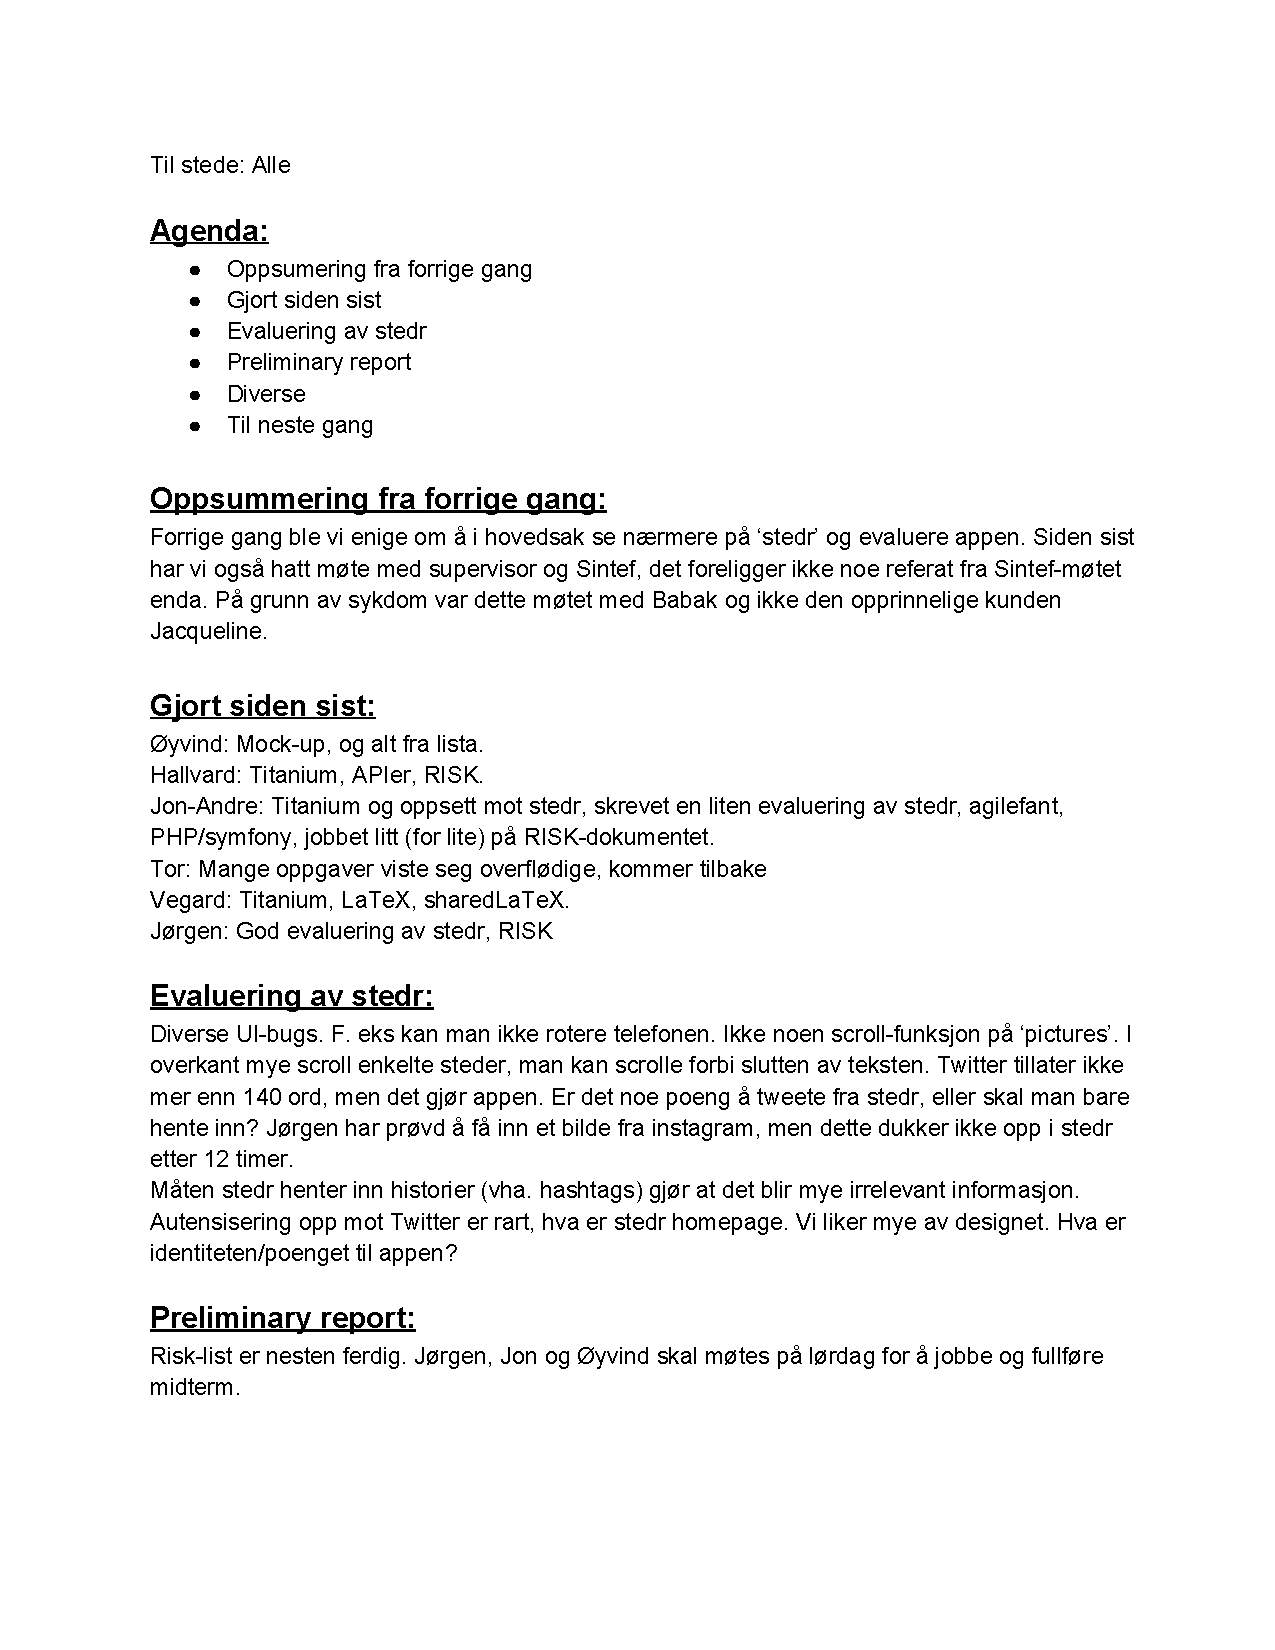
\includepdf[pages={1,2}]{res/Motereferat_05-02-14.pdf}

\subsection{Customer Meeting}
Here is an example of the summary of a meeting with our customer. Again the text is in Norwegian.
\clearpage
\begin{tikzpicture}[remember picture, overlay]
	\draw[line width = 1pt] ($(current page.north west) + (0.5in,-0.5in)$) rectangle ($(current page.south east) + (-0.5in,0.5in)$);
\end{tikzpicture}

\textbf{Videomøte med Jacqueline 19.02.2014}\\

	Til stede fra gruppe: Øyvind, Jørgen og Jon-Andre \\
	Fra kunde: Jacqueline Floch\\

Gruppa har fått mye informasjon, men hva synes Sintef er viktigst? \\
\begin{enumerate}
\item APIet til Digitalt Fortalt
\item Stable bilder til samme sted.
\item Gjøre appen bedre og forbedre integrasjonen mot eksisterende APIer.
\item Skape interesse gjennom sosiale medier (link til fortelling f. eks)
\item Filtrering
\item Koble til andre databaser (Soundcloud)
\end{enumerate}

Vil beholde så mye som mulig av det som allerede finnes i appen. Det ble brukt mye tid på design i høst, så dette bør ikke prioriteres nå.

Filtrering: Når et sted blir hentet kan man f. eks få en liste med tags. Filtrering basert på brukerprofil (og generelt) vil for øyeblikket være litt problematisk grunnet få fortellinger.  

DF har link til Wikipedia.

Hvis vi har forslag til forandring både backend/frontend så kan dette gjennomføres.

Informerer om den lille brukerundersøkelsen vi har hatt, og at vi har et inntrykk av at den sosiale delen. 

Flickr API: Et sted er definert som et bilde, geolokasjon, bilde er delt innenfor en gruppe. Gruppe-APIet til Flickr er ikke optimalt, gruppe er brukt for å gjøre søket enklere. Backend henter alle bilder og informasjon fra den gruppa.

Gruppa har et inntrykk av at appen ved førstegangsbruk er litt vanskelig, kanskje det bør være innlagt en sidemeny.

En litt abstrakt utfordring er: Hva er et sted, og hvor stort er et sted?

\textbf{Notiser:}\\
 	-Det APIet som ble brukt i høst fungerer ikke nå\\
	-Gruppa bør sjekke ut Trondheim Byguide\\

\clearpage

\subsection{Supervisor Meeting}
Here are some notes from one of our meetings with the our supervisor Mohsen Anvaari. 
We found these meetings to be a great resource during our project, giving us constructive criticism and advice. This specific meeting occurred 18.02.2014.

\clearpage
\begin{tikzpicture}[remember picture, overlay]
	\draw[line width = 1pt] ($(current page.north west) + (0.5in,-0.5in)$) rectangle ($(current page.south east) + (-0.5in,0.5in)$);
\end{tikzpicture}

\textbf{Meeting with Supervisor 18.02.2014}\\

He thought the report was generally good, but some small things were missing:

In the introduction we should have given a short introduction to the customer.

He had some issues with the structure of the report:

The term Software Engineering is too broad.
Should rather be split up in sections like Architecture, Design etc. 
An alternative would be to simply split the structure in to Sprint 1, 2 etc.

Time organization should just be called Project Planning.

Never use “things” in the report. Be more specific.

“GUI and APIs” - For what? Specify that we will work on Stedrs GUI and API.

Remember to give an brief description on what the application is for. Explain the usage.

Process is fine.

Time-plan and architecture is fine, but needs to be more detailed for the next version. 

Some of the Non-functional-reqs is functional. ISO standard. Chose 3 or 4. How we tackled it later. Diary is functional.

Linking is superimportant!

Risk analysis is very good.

\clearpage



